\documentclass{article}

\usepackage{natbib}

\usepackage[french]{babel}
\usepackage[T1]{fontenc}
\usepackage{lmodern}

\usepackage[margin=3cm]{geometry}
%\usepackage[left=0.6in,right=0.6in,top=0.6in,bottom=0.6in]{geometry}
\usepackage{graphicx}
\usepackage{multicol}
\usepackage{fancyhdr}
\usepackage{minted} 
\usepackage{hyperref}                 
\usepackage{titlesec}
\usepackage{amsfonts}
\usepackage{amsmath}

\title{ \textbf{Rapport : Affectation des étudiants en Master}\\
      \vspace{0.3cm}
      \large Implémentation de Gale-Shapley et résolution par programmation linéaire.}
\author{Jesus Alejandro Gomez Urzua\\Nadhir Ben Said}

\begin{document}
\maketitle
\tableofcontents
\vspace{0.3cm}

\section{Introduction}

Ce projet porte sur l'étude et la résolution du problème de l'affectation des étudiants au sein 
des différents parcours de Master. L'objectif est de coupler $n$ étudiants à $m$ formations en tenant 
compte de leurs préférences respectives, tout en respectant les capacités d'accueil limitées propres 
à chaque Master. L'enjeu majeur réside dans l'implémentation d'algorithmes capables de satisfaire simultanément 
plusieurs critères :  
\begin{enumerate}
      \item Stabilité : garantir qu'aucun couple (étudiant, Master) n'ait intérêt à rompre l'affectation 
      actuelle pour se choisir mutuellement.
      \item Efficacité : maximiser le bien-être total des participants selon une approche utilitariste.
      \item Équité : assurer un niveau de satisfaction minimal pour tous les agents suivant une approche égalitariste.
\end{enumerate}  
Pour ce faire, nous proposons dans un premier temps une implémentation de l'algorithme de Gale-Shapley, 
qui garantit l'obtention d'un mariage stable sans toutefois assurer l'efficacité ou l'équité de la solution. 
Dans un second temps, nous utiliserons la programmation linéaire afin d'optimiser les critères d'efficacité 
et d'équité, indépendamment des contraintes de stabilité.  

\section{Algorithme de Gale-Shapley}

L'algorithme de Gale-Shapley repose sur une stratégie de type \og propositions et rejets \fg{} 
qui garantit l'obtention d'un mariage stable. La version implémentée dans ce projet adapte 
le modèle vu en cours pour intégrer les capacités d'accueil des Masters. Dans cette configuration, 
un parcours accepte une proposition tant qu'il dispose de places vacantes. Une fois sa capacité 
atteinte, il ne valide une nouvelle candidature que si l'étudiant proposant est mieux classé que 
l'étudiant le moins préféré parmi ceux déjà acceptés.


\subsection{Optimisation avec des structures de données}
Afin de garantir une complexité efficace, nous avons couplé chaque opération élémentaire de 
l'algorithme à une structure de données adaptée :

\begin{enumerate}
      \item \textbf{Identification des étudiants libres :} L'utilisation d'une \texttt{deque} permet d'extraire 
      un étudiant et de le réinsérer en cas de rejet en $\mathcal{O}(1)$.  
      
      \item \textbf{Sélection du prochain parcours :} Un tableau d'entiers mémorise pour chaque étudiant l'indice 
      du prochain Master à solliciter dans sa liste de préférences, garantissant une sélection en $\mathcal{O}(1)$.
  
      \item \textbf{Évaluation du rang :} Le pré-calcul d'une matrice des rangs en $\mathcal{O}(n \times m)$ 
      permet à chaque Master de connaître en temps constant la position d'un candidat dans son classement. 
      
  
      \item \textbf{Gestion des admissions :} Chaque Master gère ses étudiants admis via un tas binaire. 
      Cette structure permet d'identifier l'étudiant le moins préféré en $\mathcal{O}(1)$ et de 
      mettre à jour l'affectation en $\mathcal{O}(\log(k))$, où $k$ est la capacité maximale 
      d'un parcours.
\end{enumerate}

Ainsi, notre implémentation atteint une complexité globale de $\mathcal{O}(n \times m \log(k))$

\subsection{Adaptation pour l'exécution côté parcours}

Il est important de noter que cet algorithme n'est pas symétrique : il favorise systématiquement 
le groupe qui émet les propositions. En l'occurrence, cette version est \textit{étudiant-optimale}, 
offrant à chaque étudiant la meilleure affectation possible parmi tous les mariages stables, tout 
en étant \textit{parcours-pessimale}.

Dans la version où les Masters proposent aux étudiants, l'implémentation se rapproche davantage du 
modèle abordé en cours et devient plus simple. En effet, la gestion des priorités par un tas binaire 
devient superflue : chaque étudiant ne pouvant être affecté qu'à un seul Master, il lui suffit de 
comparer toute nouvelle offre à son affectation actuelle pour l'accepter ou la rejeter. Pour gérer 
les capacités d'accueil, chaque Master est inséré dans la \texttt{deque} autant de fois qu'il possède 
de places disponibles. Ainsi, la somme des capacités étant égale au nombre d'étudiants, dans cette 
version la complexité de $\mathcal{O}(n^2)$. 

\subsection{Jeux de tests et analyse de performances}

\begin{figure}
      \centering
      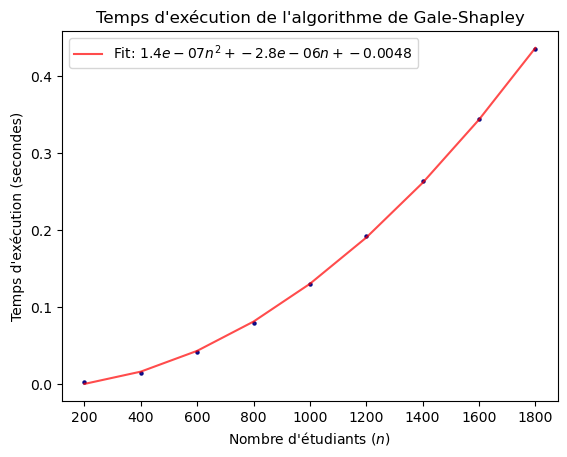
\includegraphics[width=7cm]{img/temps_moy.png}
      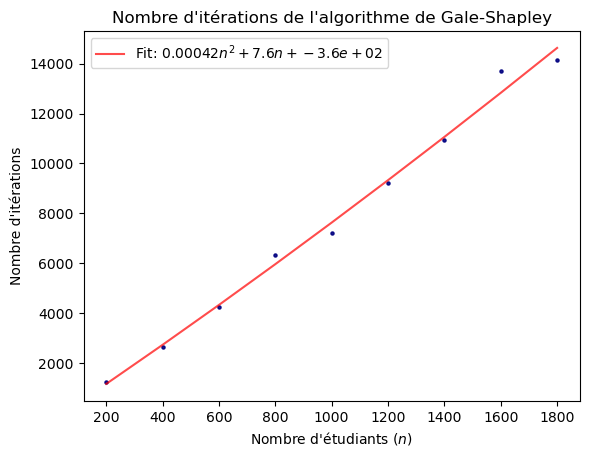
\includegraphics[width = 7cm]{img/it_moy.png}
      \caption{Exécution de l'algorithme Gale-Shapley pour des données aléatoires.}
      \label{fig:moy}
\end{figure}

La fiabilité de l'implémentation a été vérifiée par un jeu de tests via la bibliothèque 
\texttt{unittest}. Divers scénarios d'affectation ont été élaborés manuellement et stockés dans 
un fichier \texttt{JSON} incluant les résultats attendus. Ces tests couvrent l'algorithme 
de Gale-Shapley (variantes étudiant et parcours) ainsi que la fonction de détection des paires instables.

Pour confronter les performances observées à la complexité théorique, nous avons mesuré le temps 
d'exécution et le nombre d'itérations pour des instances allant de 200 à 2000 agents.

Dans un premier temps, l'algorithme a été testé sur des matrices de préférences aléatoires et uniformes. 
Les résultats dans la Figure \ref{fig:moy} montrent un temps d'exécution quadratique, alors que le nombre 
d'itérations suit une croissance plus lente. Cette observation est cohérente avec les travaux de \cite{wil72}, 
qui démontrent que le nombre moyen de propositions est en $\mathcal{O}(n \log n)$ sous l'hypothèse de 
préférences indépendantes et uniformes. La divergence entre le temps et les itérations s'explique par la 
phase de pré-calcul, dont la complexité est en $\mathcal{O}(n \times m)$ quel que soit le contenu des préférences.

Dans un second temps, nous avons soumis l'implémentation à un scénario de pire cas (Figure \ref{fig:pire}). 
Dans cette configuration, le temps de calcul et le nombre d'itérations suivent tous deux 
un comportement quadratique, confirmant ainsi la borne supérieure théorique de l'algorithme.

\begin{figure}
      \centering
      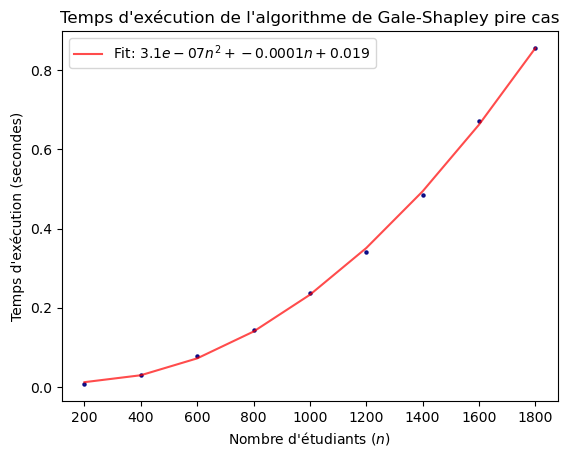
\includegraphics[width=7cm]{img/temps_pire_cas.png}
      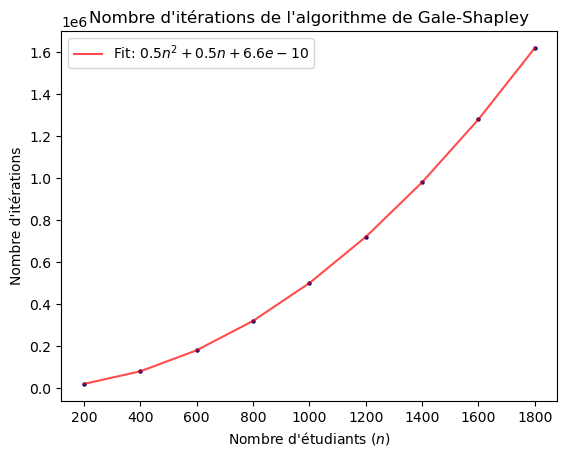
\includegraphics[width=7cm]{img/it_pire_cas.png}
      \caption{Exécution de l'algorithme Gale-Shapley avec des données forçant le pire cas.}
      \label{fig:pire}
\end{figure}


\section{Programmation Linéaire}

Cette seconde partie du projet explore l'utilisation de la programmation linéaire pour résoudre le problème 
d'affectation sous différents critères, tels que l'efficacité et l'équité.

Pour quantifier la satisfaction des agents, nous définissons l'utilité par les scores de Borda. Afin de simplifier
nos calculs, dans nos programmes linéaires, nous utiliserons directement le rang dans la matrice de préférences. Ainsi,
maximiser l'utilité revient a minimiser le rang. On note $b_{j,i}$ le rang du $i$-ème étudiant dans le $j$-ème parcours,
et $c_{i,j}$ le rang du $j$-ème parcours dans la liste de préférences du $i$ème étudiant et $C_j$ la capacité du $j$-ème
parcours.


\subsection{Maximisation de l'utilité minimale des étudiants}

Pour garantir une certaine équité, nous cherchons à minimiser le mécontentement de l'étudiant le 
plus mal loti. Nous introduisons une variable auxiliaire $z$ représentant le rang maximal
atteint par un étudiant.\\
\textbf{Variables:}
\begin{itemize}
    \item $x_{i,j} \in \{0, 1\}$ : vaut 1 si l'étudiant $i$ est affecté au Master $j$, 0 sinon.
    \item $z \in \mathbb{N}$ : le rang maximal observé.
\end{itemize}
\textbf{Fonction objectif:} $\min z$ \\
\textbf{Contraintes:}
\begin{align*}
    & \sum_{j=1}^{m} x_{i,j} = 1, & \forall i \in \{1, \dots, n\} \\
    & \sum_{j=1}^{m} c_{i,j} x_{i,j} \le z, & \forall i \in \{1, \dots, n\} \\
    & \sum_{i=1}^{n} x_{i,j} \le C_j, & \forall j \in \{1, \dots, m\} \\
\end{align*}

\subsection{Maximisation de l'utilité totale}

Le modèle précédent omettait les préférences des établissements. Nous cherchons désormais à 
maximiser l'efficacité globale en optimisant la somme des utilités des étudiants et des parcours 
(approche utilitariste).

\textbf{Variables:}
\begin{itemize}
    \item $x_{i,j} \in \{0, 1\}$ : vaut 1 si l'étudiant $i$ est affecté au Master $j$, 0 sinon.
\end{itemize}
\textbf{Fonction objectif:} $\min \sum_{i=1}^n \sum_{j=1}^m x_{i,j} (b_{i,j}+c_{i,j})$ \\
\textbf{Contraintes:}
\begin{align*}
    & \sum_{j=1}^{m} x_{i,j} = 1, & \forall i \in \{1, \dots, n\} \\
    & \sum_{i=1}^{n} x_{i,j} \le C_j, & \forall j \in \{1, \dots, m\} \\
\end{align*}


\subsection{Optimisation sous contrainte de rang}

Cette variante maximise l'utilité totale tout en garantissant à chaque étudiant une affectation 
parmi ses $k$ premiers vœux. 

\textbf{Variables:}
\begin{itemize}
    \item $x_{i,j} \in \{0, 1\}$ : vaut 1 si l'étudiant $i$ est affecté au Master $j$, 0 sinon.
\end{itemize}
\textbf{Fonction objectif:} $\min \sum_{i=1}^n \sum_{j=1}^m x_{i,j} (b_{i,j}+c_{i,j})$ \\
\textbf{Contraintes:}
\begin{align*}
    & \sum_{j=1}^{m} x_{i,j} = 1, & \forall i \in \{1, \dots, n\} \\
    & \sum_{i=1}^{n} x_{i,j} \le C_j, & \forall j \in \{1, \dots, m\} \\
    & \sum_{j=1}^{m} c_{i,j} x_{i,j} \leq k, & \forall i \in \{1, \dots, n\} \\
\end{align*}

\section{Analyse comparative}

\begin{table}
      \footnotesize
      \centering
      \begin{tabular}{|c c c c c c|}
            \hline
            Étudiant & GS côté étudiants & GS côté parcours & Max min util & Max util totale & Max util totale $k=5$\\
            \hline \hline
            0  & 5 & 5 & 9 & 8 & 8 \\
            1  & 6 & 6 & 6 & 5 & 5 \\
            2  & 9 & 9 & 2 & 4 & 4 \\
            3  & 9 & 9 & 9 & 9 & 9 \\
            4  & 1 & 1 & 1 & 1 & 1 \\
            5  & 0 & 0 & 4 & 0 & 9 \\
            6  & 8 & 8 & 7 & 7 & 7 \\
            7  & 7 & 7 & 0 & 0 & 0 \\
            8  & 3 & 3 & 5 & 9 & 6 \\
            9  & 2 & 2 & 8 & 2 & 2 \\
            10 & 4 & 4 & 3 & 4 & 3 \\
            11 & 4 & 4 & 4 & 3 & 4 \\
            12 & 0 & 0 & 0 & 6 & 0\\
            \hline
      \end{tabular}
      \caption{Récapitulatif des affectations par méthode pour chaque étudiant.}
      \label{tab:aff}
\end{table}

\begin{table}
      \centering
      \footnotesize
      \begin{tabular}{|c | c c c c c|}
            \hline
            Métrique & GS côté étudiants & GS côté parcours & Max min util & Max util totale & Max util totale $k=5$\\
            \hline \hline
            Somme des utilités            & 203  & 203   & 178  & 213   & 201 \\
            Utilité moyenne (étudiants)   & 7.84 & 7.84  & 7.61 & 7.15  & 7.84\\
            Utilité moyenne (parcours)    & 7.76 & 7.76  & 6.07 & 9.23  & 7.61\\
            Utilité minimale (étudiants)  & 4    & 4     & 5    & 0     & 5 \\
            Utilité minimale (parcours)   & 0    & 0     & 0    & 0     &  0 \\
            Paires instables              & 0    & 0     & 9    & 7     & 5 \\
            \hline
      \end{tabular}
      \caption{Analyse comparative des indicateurs de performance.}
      \label{tab:ut}
\end{table}

Afin d'évaluer les différentes méthodes étudiées, nous les avons appliquées au jeu de données fourni. 
Les affectations obtenues sont consignées dans le Tableau \ref{tab:aff}.

Nous avons analysé ces résultats selon des indicateurs de stabilité (nombre de paires instables),
 d'équité (utilités maximale et moyenne des étudiants) et d'efficacité (somme totale des utilités). 
 Le Tableau \ref{tab:ut} synthétise ces mesures, permettant ainsi d'apprécier les compromis entre stabilité, 
 satisfaction globale et équité propres à chaque modèle.

\bibliographystyle{agsm}
\bibliography{references}

\end{document}